
\Section{Payment channels}
A payment channel is a channel where transactions can be exchanged trustlessly on channels other than directly on the blockchain.
This is what is sually refered to as off-chain transactions.
In their most naive form a payment channel can simply be Alice and Bob exchanging promises of future transactions later.
This however is not trustless and any of the parties could later withdraw from the promise without punishment (other than maybe loss of friendship).

To build a trustless payment channel there are several ways to go about as Script is quite versatile.
The method that will be covered here uses a type of channel \textbf{funding transaction that requires the signature from both parties to spend}, and the channel balance is updated via special commitment transactions that spend the funding output. Each party in the channel has their own version of the commitment transaction. Whenever a commitment transaction is broadcast to the blockchain the channel is closed as the funding transaction can't be spent twice. To update the balance in the channel both parties create new commitment transactions and signs the other parties commitment transaction.  
Let's take a look at a naive example:

\Subsubsection{The naive payment channel}
Imagine Alice and Bob wants to open a payment channel between eachother. They create a funding transaction and the initial commitment transactions. Let's say they both funded the channel with 1 Bitcoin each. The initial commitment transactions would then have one output paying 1 Bitcoin to Alice and one output paying 1 Bitcoin to Bob, let's call this commit (\textbf{C0}).
The funding transaction is braodcast to the blockchain.

A bit later Alice buys one funny hat from Bob for 0.1 Bitcoins. To complete the transaction they create two new commitment transaction that pays 0.9 Bitcoin to Alice and 1.1 Bitcoin to Bob and signs them for each other, let's call this new commitment (\textbf{C1}). Any number of transactions could be exhanged this way. The channel could be closed by any one broadcasting their commitment transaction. This naive implementation of a payment channel has a fatal flaw however. 

A payment channel needs some safety measures to be safe from malicious actors. The above example lacks a mechanism for preventing old commitment transactions from making their way into the blockchain and still paying the malicious party.. For example after the initial funny hat transaction above (\textbf{C1}) Alice could just broadcast the initial commit transaction (\textbf{C0}) and reclaim the 0.1 Bitcoins she spent. Bob would have no way of preventing this in this naive implementation.

\Subsubsection{Transaction flow diagrams}
The transactions that are involved in making payment channels grows larger the more features that are added. To make it easier to understand, diagrams are used together with the descriptions. In Figure \ref{fig:anatomy} a basic overview of the diagram-realm transaction is shown. Lines leading from outputs to inputs means that the connected input are spending that output. Note that one output can be connected to several inputs but each input can only be connected to one output, of course an output can only be spent once, this will be clarified later. A \textbf{?} in the broadcaster field indicates either that the sender is unknown or that who sends it is irrelevant. 


\begin{figure}[H]
	\centering
	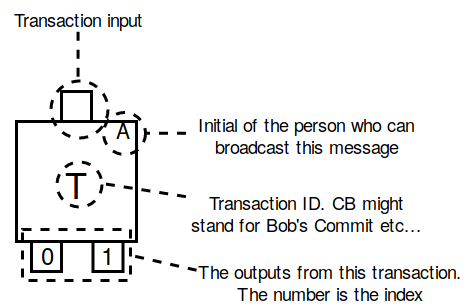
\includegraphics[width=0.5\textwidth]{background/images/tx_anatomy.png}
	\caption{Different parts of a transaction as they appear in diagrams.}
	\label{fig:anatomy}
\end{figure}

\Subsubsection{Payment channel with breach remedy}
To prevent old transactions from being sent to the blockchain a new mechanism needs to be devised. This can be done via something called revocable delivery and breach remedy (Some times called just revocation).
Instead of both parties holding the same commit. They each get an individual one that differs in it's outputs. 


\begin{figure}[H]
	\centering
	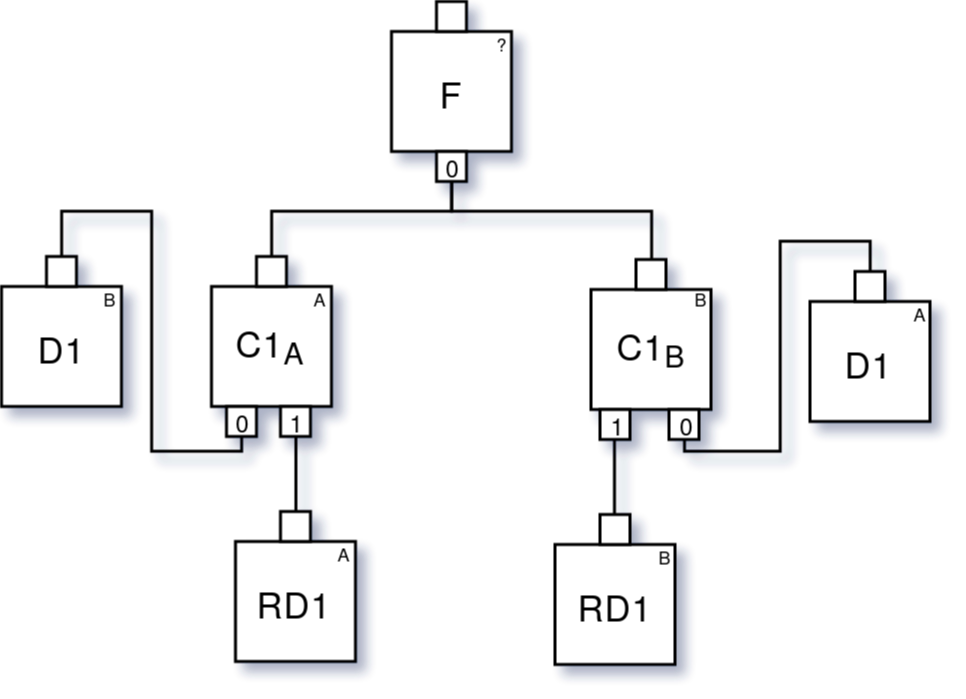
\includegraphics[width=0.6\textwidth]{background/images/payment_channel_pre_breach.png}
	\caption{Payment channel, with commits using revocable delivery mechanism}
	\label{fig:pre-breach}
\end{figure}

Figure \ref{fig:pre-breach} shows how the payment channel appears after the first commitment transactions has been made. Let's say the channel is between Alice (A) and Bob (B) and the balance in the channel is 0.5 BTC for Alice and 0.5 BTC for Bob. 

\textbf{$C1_{A}$} is the commitment transaction on Alice's side of the channel. As with all commitment transactions it spends the funding transaction. It has two outputs. One sending 0.5 BTC